\documentclass{ximera}


\input{../../../preamble.tex}


\definecolor{fvdnavy}{HTML}{071D43}
\definecolor{fvdcyan}{HTML}{20BFC6}
\definecolor{fvdcyanlight}{HTML}{EFFCFB}
\definecolor{fvdmagenta}{HTML}{F10D69}
\definecolor{fvdmagentalight}{HTML}{FFF1F7}
\definecolor{fvdtext}{HTML}{163044}





%=================================================
% Pedagogische omgevingen
% PDF: tcolorbox
% HTML: learning-box
%=================================================

\newenvironment{voorkennis}
{%
    \ifdefined\HCode
        \HCode{%
<section class="learning-box learning-box--prior">
<div class="learning-box__header">
<span class="learning-box__icon" aria-hidden="true"></span>
<span class="learning-box__title">Voorkennis</span>
</div>
<div class="learning-box__content">
        }%
        \begin{itemize}
    \else
       \begin{tcolorbox}[
    enhanced,
    breakable,
    colback=fvdcyanlight,
    colframe=fvdcyan,
    coltext=fvdtext,
    boxrule=0.5pt,
    leftrule=4pt,
    arc=4mm,
    outer arc=4mm,
    left=7mm,
    right=6mm,
    top=5mm,
    bottom=5mm,
    before skip=6mm,
    after skip=6mm,
    title=Voorkennis,
    coltitle=fvdcyan,
    fonttitle=\bfseries\Large,
    attach title to upper={\par\smallskip},
    boxed title style={
        empty,
        left=0mm,
        right=0mm,
        top=0mm,
        bottom=0mm
    },
    overlay={
        \draw[
            fvdcyan,
            line width=0.5pt
        ]
        ([xshift=42mm,yshift=-13mm]frame.north west)
        --
        ([xshift=-7mm,yshift=-13mm]frame.north east);
    }
]
        \begin{itemize}
    \fi
}
{%
    \end{itemize}
    \ifdefined\HCode
        \HCode{%
</div>
</section>
        }%
    \else
        \end{tcolorbox}
    \fi
}


\newenvironment{leerdoelen}
{%
    \ifdefined\HCode
        \HCode{%
<section class="learning-box learning-box--goals">
<div class="learning-box__header">
<span class="learning-box__icon" aria-hidden="true"></span>
<span class="learning-box__title">Leerdoelen</span>
</div>
<div class="learning-box__content">
        }%
        \begin{itemize}
    \else
\begin{tcolorbox}[
    enhanced,
    breakable,
    colback=fvdmagentalight,
    colframe=fvdmagenta,
    coltext=fvdtext,
    boxrule=0.5pt,
    leftrule=4pt,
    arc=4mm,
    outer arc=4mm,
    left=7mm,
    right=6mm,
    top=5mm,
    bottom=5mm,
    before skip=6mm,
    after skip=6mm,
    title=Leerdoelen,
    coltitle=fvdmagenta,
    fonttitle=\bfseries\Large,
    attach title to upper={\par\smallskip},
    boxed title style={
        empty,
        left=0mm,
        right=0mm,
        top=0mm,
        bottom=0mm
    },
    overlay={
        \draw[
            fvdmagenta,
            line width=0.5pt
        ]
        ([xshift=42mm,yshift=-13mm]frame.north west)
        --
        ([xshift=-7mm,yshift=-13mm]frame.north east);
    }
]
        \begin{itemize}
    \fi
}
{%
    \end{itemize}
    \ifdefined\HCode
        \HCode{%
</div>
</section>
        }%
    \else
        \end{tcolorbox}
    \fi
}



\title{Rekenen met gehele getallen}


\begin{document}

% FVD_CHAPTER_DATA_START
% Automatisch gegenereerd uit index.tex.
% Niet handmatig aanpassen.
\fvdchapterdata{1}{Rekenen met inzicht}{1}
% FVD_CHAPTER_DATA_END


\begin{abstract}
    In dit hoofdstuk leer je gehele getallen begrijpen en correct gebruiken.
    Je oefent de vier hoofdbewerkingen, rekent met positieve en negatieve
    getallen en ontwikkelt strategieën om eenvoudige berekeningen vlot uit
    het hoofd uit te voeren.
    \end{abstract}

\maketitle

% ============================================================
% VOORKENNIS EN LEERDOELEN
% ============================================================

\begin{voorkennis}
    \item Je kan eenvoudige getallen lezen en vergelijken;
    \item Je herkent de symbolen \(+\), \(-\), \(\times\) en \(\div\).
    \item Je kan eenvoudige optellingen en aftrekkingen kunt uitvoeren.
    \item Je kan een getallenlijn kunt aflezen.
\end{voorkennis}

\begin{leerdoelen}
    \item Je kan natuurlijke en gehele getallen herkennen.
    \item Je kan positieve en negatieve getallen vergelijken en ordenen.
    \item Je kan gehele getallen voorstellen op een getallenlijn.
    \item Je kan gehele getallen optellen, aftrekken, vermenigvuldigen en delen.
    \item Je kan eenvoudige berekeningen vlot uit het hoofd uitvoeren.
    \item Je kan een geschikte hoofdrekenstrategieën gebruiken.
    \item Je kan de tafels en deeltafels toepassen in berekeningen.
    \item Je an vooraf inschatten hoe groot een antwoord ongeveer moet zijn.
    \item Je kan controleren of een antwoord logisch is.
\end{leerdoelen}

\FVDStartPositionFigure{-6}{6}{5}

%%%%%%%%%%%%%%%%%%%%%%%%%%%%%%%%%%%%%%%%%%%%%%%%%%%%%%%%%%%%
%% WAAROM LEER JE DIT?
%%%%%%%%%%%%%%%%%%%%%%%%%%%%%%%%%%%%%%%%%%%%%%%%%%%%%%%%%%%%

\FVDsection{Waarom leer je dit?}

Een computer kan miljoenen berekeningen per seconde uitvoeren.
Toch begrijpt hij niet vanzelf wat jij bedoelt. Hij voert alleen de
instructies uit die jij invoert.

Een kleine rekenfout kan daardoor grote gevolgen hebben:

\begin{itemize}
  \item een personage verschijnt op de verkeerde plaats;
  \item een score wordt verkeerd berekend;
  \item een object beweegt in de verkeerde richting;
  \item een animatie duurt te lang of te kort;
  \item een programma geeft een onverwacht resultaat.
\end{itemize}

Daarom moet je eenvoudige berekeningen niet alleen kunnen uitvoeren,
maar ook kunnen inschatten of een resultaat logisch is.

\begin{voorbeeld}
    Stel dat een personage op positie \(8\) staat en \(3\) stappen naar links
beweegt. Dan verwacht je een positie kleiner dan \(8\). Geeft je berekening
als antwoord \(11\), dan weet je meteen dat er iets fout is gegaan.
\end{voorbeeld}


Vlot rekenen helpt je dus niet alleen sneller te werken. Het helpt je ook
om fouten te herkennen, formules beter te begrijpen en later gemakkelijker
te werken met algebra, functies, coördinaten en vectoren.


\begin{themaintro}{Rekenvaardigheid groeit door oefening}

    Om later vlot te kunnen werken met formules en digitale toepassingen,
    moeten enkele basisberekeningen voldoende geautomatiseerd zijn.
    
    Daarbij horen onder andere:
    
    \begin{itemize}
      \item optellingen en aftrekkingen met kleine getallen;
      \item de tafels van vermenigvuldiging;
      \item de bijbehorende deeltafels;
      \item eenvoudige berekeningen met negatieve getallen;
      \item slim rekenen door te splitsen, aan te vullen of te compenseren.
    \end{itemize}
    
    Lukt dit nog niet helemaal uit het hoofd? Dat is geen probleem.
    In dit hoofdstuk en in de volgende hoofdstukken vind je regelmatig een
    \textbf{Rekenfitness}. Daarin train je deze vaardigheden kort maar vaak.
    
    Net zoals bij sporten word je niet sterker door één lange training,
    maar door regelmatig te oefenen.
    
    \end{themaintro}

%%%%%%%%%%%%%%%%%%%%%%%%%%%%%%%%%%%%%%%%%%%%%%%%%%%%%%%%%%%%%%%%%%%%%%
%% ONTDEKKEN
%%%%%%%%%%%%%%%%%%%%%%%%%%%%%%%%%%%%%%%%%%%%%%%%%%%%%%%%%%%%%%%%%%%%%%

\section{Ontdekken}

\begin{exploration}{Waar staat het personage?}

Bij het ontwikkelen van een computerspel krijgt elk object een plaats
in de digitale wereld. Die plaats wordt beschreven met getallen.

Stel dat een personage zich over een rechte weg beweegt. We spreken af dat:

\begin{itemize}
  \item bewegen naar rechts een positieve beweging is;
  \item bewegen naar links een negatieve beweging is.
\end{itemize}

Het personage start op positie \(5\).

\FVDStartPositionFigure{-6}{6}{5}

Voer nu achtereenvolgens de volgende bewegingen uit:

\begin{enumerate}
  \item \(3\) stappen naar links;
  \item \(7\) stappen naar rechts;
  \item \(12\) stappen naar links.
\end{enumerate}

\begin{question}
Op welke positie bevindt het personage zich na de eerste beweging?
\end{question}

\begin{question}
Op welke positie bevindt het personage zich na de tweede beweging?
\end{question}

\begin{question}
Waar bevindt het personage zich uiteindelijk?
\end{question}

\begin{question}
Kan een positie kleiner zijn dan nul? Leg uit in je eigen woorden.
\end{question}

\end{exploration}

%%%%%%%%%%%%%%%%%%%%%%%%%%%%%%%%%%%%%%%%%%%%%%%%%%%%%%%%%%%%%%%%%%%%%%
%% WAT MERK JE?
%%%%%%%%%%%%%%%%%%%%%%%%%%%%%%%%%%%%%%%%%%%%%%%%%%%%%%%%%%%%%%%%%%%%%%

\FVDsection{Wat merk je?}

Wanneer je alle bewegingen uitvoert, eindigt het personage links van nul.

Dat is vreemd, want bij het tellen gebruiken we meestal enkel de getallen

\[
0,\;1,\;2,\;3,\;4,\ldots
\]

Blijkbaar hebben we ook getallen nodig die \textbf{kleiner zijn dan nul}.

Die noemen we \textbf{negatieve getallen}.

Samen met nul en de positieve getallen vormen ze de
\textbf{gehele getallen}.


%%%%%%%%%%%%%%%%%%%%%%%%%%%%%%%%%%%%%%%%%%%%%%%%%%%%%%%%%%%%%%%%%%%%%%
%% GEHELE GETALLEN
%%%%%%%%%%%%%%%%%%%%%%%%%%%%%%%%%%%%%%%%%%%%%%%%%%%%%%%%%%%%%%%%%%%%%%

\FVDsection{Gehele getallen}

De gehele getallen liggen allemaal op één rechte lijn.

\begin{center}
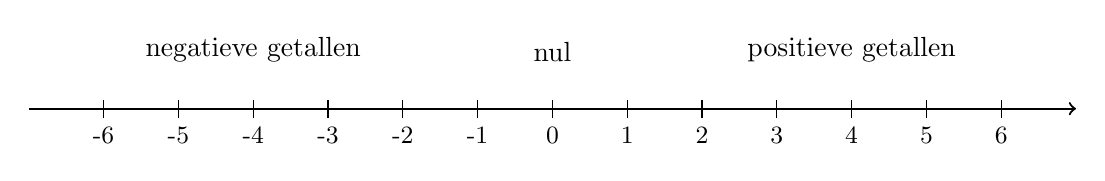
\begin{tikzpicture}[scale=0.95]

\draw[->,thick] (-7,0)--(7,0);

\foreach \x in {-6,...,6}
{
\draw (\x,0.12)--(\x,-0.12);
\node[below] at (\x,-0.12){\small \x};
}

\node[above] at (-4,0.5){negatieve getallen};

\node[above] at (0,0.5){nul};

\node[above] at (4,0.5){positieve getallen};

\end{tikzpicture}
\end{center}

Alle getallen op deze getallenlijn noemen we de
\textbf{gehele getallen}.

We noteren deze verzameling met

\[
\mathbb Z.
\]

Enkele voorbeelden zijn

\[
-8,\;
-3,\;
0,\;
5,\;
14.
\]

%%%%%%%%%%%%%%%%%%%%%%%%%%%%%%%%%%%%%%%%%%%%%%%%%%%%%%%%%%%%%%%%%%%%%%
%% NATUURLIJKE GETALLEN
%%%%%%%%%%%%%%%%%%%%%%%%%%%%%%%%%%%%%%%%%%%%%%%%%%%%%%%%%%%%%%%%%%%%%%

\FVDsection{Natuurlijke getallen}

Wanneer we tellen, gebruiken we meestal alleen de natuurlijke getallen.

\[
0,\;1,\;2,\;3,\;4,\;5,\ldots
\]

Deze verzameling noteren we met

\[
\mathbb N.
\]

De natuurlijke getallen maken dus deel uit van de gehele getallen.

\[
\mathbb N \subset \mathbb Z
\]

%%%%%%%%%%%%%%%%%%%%%%%%%%%%%%%%%%%%%%%%%%%%%%%%%%%%%%%%%%%%%%%%%%%%%%
%% VOORBEELDEN
%%%%%%%%%%%%%%%%%%%%%%%%%%%%%%%%%%%%%%%%%%%%%%%%%%%%%%%%%%%%%%%%%%%%%%

\FVDsection{Positieve en negatieve getallen}

Negatieve getallen komen voortdurend voor in digitale toepassingen.

\begin{example}
In een computerspel bevindt een object zich op positie

\[
x=-4.
\]

Dat betekent dat het object vier eenheden links van de oorsprong staat.
\end{example}

\begin{example}
Een camera bevindt zich op hoogte

\[
y=3.
\]

Ze wordt vijf eenheden naar beneden verplaatst.

Wat is de nieuwe hoogte?

\[
3-5=-2
\]

De camera bevindt zich nu twee eenheden onder het referentiepunt.
\end{example}


%%%%%%%%%%%%%%%%%%%%%%%%%%%%%%%%%%%%%%%%%%%%%%%%%%%%%%%%%%%%%%%%%%%%%%
%% DENKVRAAG
%%%%%%%%%%%%%%%%%%%%%%%%%%%%%%%%%%%%%%%%%%%%%%%%%%%%%%%%%%%%%%%%%%%%%%

\begin{question}

    Drie objecten bevinden zich op de volgende plaatsen.
    
    \[
    A(-6),\qquad
    B(-2),\qquad
    C(4)
    \]
    
    \begin{enumerate}
    \item Welk object ligt het meest links?
    \item Welk object ligt het dichtst bij nul?
    \item Welk object ligt het meest rechts?
    \end{enumerate}
    
    \end{question}

% ============================================================
\FVDsection{Tegengestelde getallen en absolute waarde}
% ============================================================

Twee getallen zijn \textbf{tegengesteld} wanneer ze even ver van nul liggen,
maar aan een andere kant van nul.

Voorbeelden:

\[
5 \text{ en } -5,
\qquad
-12 \text{ en } 12.
\]

Het tegengestelde van een getal $a$ is $-a$.

\begin{example}
Het tegengestelde van $-7$ is

\[
-(-7)=7.
\]
\end{example}

De \textbf{absolute waarde} van een getal is de afstand van dat getal tot nul.
Een afstand is nooit negatief.

De absolute waarde van $a$ wordt genoteerd als $|a|$.

\[
|5|=5,
\qquad
|-5|=5,
\qquad
|0|=0.
\]

\begin{exercise}
Bereken.

\begin{enumerate}
    \item $|-9|=\answer{9}$
    \item $|4|=\answer{4}$
    \item $-|-6|=\answer{-6}$
    \item $|-3|+|5|=\answer{8}$
\end{enumerate}
\end{exercise}

% ============================================================
\FVDsection{Optellen met gehele getallen}
% ============================================================

\xmsubsection{Getallen met hetzelfde teken}

Wanneer beide getallen hetzelfde teken hebben:

\begin{enumerate}
    \item tel je de absolute waarden op;
    \item behoud je het gemeenschappelijke teken.
\end{enumerate}

\begin{example}
\[
7+5=12.
\]
\end{example}

\begin{example}
\[
-7+(-5)=-12.
\]
\end{example}

\xmsubsection{Getallen met een verschillend teken}

Wanneer de getallen een verschillend teken hebben:

\begin{enumerate}
    \item trek je de kleinste absolute waarde af van de grootste;
    \item neem je het teken van het getal met de grootste absolute waarde.
\end{enumerate}

\begin{example}
\[
8+(-3)=5.
\]

Omdat $|8|>|-3|$, is het resultaat positief.
\end{example}

\begin{example}
\[
-11+4=-7.
\]

Omdat $|-11|>|4|$, is het resultaat negatief.
\end{example}

\xmsubsection{Denken als een verplaatsing}

Je kunt een optelling voorstellen als een verplaatsing op de getallenas.

\begin{itemize}
    \item een positief getal: naar rechts;
    \item een negatief getal: naar links.
\end{itemize}

\begin{example}
\[
-3+7=4.
\]

Start bij $-3$ en verplaats $7$ plaatsen naar rechts.
\end{example}

\begin{exercise}
Bereken zonder rekenmachine.

\begin{enumerate}
    \item $6+9=\answer{15}$
    \item $-6+(-9)=\answer{-15}$
    \item $12+(-5)=\answer{7}$
    \item $-12+5=\answer{-7}$
    \item $-8+8=\answer{0}$
    \item $17+(-23)=\answer{-6}$
\end{enumerate}
\end{exercise}

% ============================================================
\FVDsection{Aftrekken met gehele getallen}
% ============================================================

Een aftrekking kun je altijd omzetten in een optelling met het tegengestelde.

\[
a-b=a+(-b).
\]

Dit is de belangrijkste regel voor aftrekken met negatieve getallen.

\begin{example}
\[
8-3=8+(-3)=5.
\]
\end{example}

\begin{example}
\[
8-(-3)=8+3=11.
\]
\end{example}

\begin{example}
\[
-5-7=-5+(-7)=-12.
\]
\end{example}

\begin{example}
\[
-5-(-7)=-5+7=2.
\]
\end{example}

\xmsubsection{Praktische werkwijze}

Bij een aftrekking:

\begin{enumerate}
    \item laat het eerste getal staan;
    \item verander het minteken van de bewerking in een plusteken;
    \item vervang het tweede getal door zijn tegengestelde;
    \item voer de optelling uit.
\end{enumerate}

\[
-9-(-4)
=
-9+4
=
-5.
\]

\begin{exercise}
Bereken.

\begin{enumerate}
    \item $9-4=\answer{5}$
    \item $9-(-4)=\answer{13}$
    \item $-9-4=\answer{-13}$
    \item $-9-(-4)=\answer{-5}$
    \item $4-11=\answer{-7}$
    \item $-6-(-10)=\answer{4}$
\end{enumerate}
\end{exercise}

% ============================================================
\FVDsection{Vermenigvuldigen en delen}
% ============================================================

Bij vermenigvuldigen en delen bepaal je eerst het teken van het resultaat.

\[
\begin{array}{c|c}
\text{tekens} & \text{teken van het resultaat} \\ \hline
+\text{ en }+ & + \\
-\text{ en }- & + \\
+\text{ en }- & - \\
-\text{ en }+ & -
\end{array}
\]

Kort samengevat:

\begin{center}
\textbf{Gelijke tekens geven plus. Verschillende tekens geven min.}
\end{center}

\begin{example}
\[
(-4)\cdot 6=-24.
\]
\end{example}

\begin{example}
\[
(-4)\cdot(-6)=24.
\]
\end{example}

\begin{example}
\[
42:(-7)=-6.
\]
\end{example}

\begin{example}
\[
(-42):(-7)=6.
\]
\end{example}

\begin{exercise}
Bereken.

\begin{enumerate}
    \item $7\cdot(-5)=\answer{-35}$
    \item $(-7)\cdot(-5)=\answer{35}$
    \item $48:(-6)=\answer{-8}$
    \item $(-48):(-6)=\answer{8}$
    \item $0\cdot(-15)=\answer{0}$
    \item $-81:9=\answer{-9}$
\end{enumerate}
\end{exercise}

% ============================================================
\FVDsection{De volgorde van bewerkingen}
% ============================================================

Wanneer een berekening verschillende bewerkingen bevat, voer je die niet zomaar
van links naar rechts uit.

Gebruik deze volgorde:

\begin{enumerate}
    \item \textbf{haakjes};
    \item \textbf{machten en wortels};
    \item \textbf{vermenigvuldigen en delen}, van links naar rechts;
    \item \textbf{optellen en aftrekken}, van links naar rechts.
\end{enumerate}

Een mogelijk geheugensteuntje is:

\[
\boxed{\text{H -- M -- V/D -- O/A}}
\]

\xmsubsection{Voorbeeld zonder haakjes}

\begin{example}
Bereken:
\[
7+3\cdot 4.
\]

Eerst de vermenigvuldiging:

\[
7+3\cdot4
=
7+12
=
19.
\]
\end{example}

\xmsubsection{Voorbeeld met delen en aftrekken}

\begin{example}
\[
20-12:3
=
20-4
=
16.
\]
\end{example}

\xmsubsection{Bewerkingen van gelijke rang}

Vermenigvuldigen en delen hebben dezelfde voorrang. Je werkt dan van links naar
rechts.

\begin{example}
\[
24:6\cdot2
=
4\cdot2
=
8.
\]

Niet:

\[
24:12=2.
\]
\end{example}

Ook optellen en aftrekken hebben dezelfde voorrang.

\begin{example}
\[
10-6+2
=
4+2
=
6.
\]
\end{example}

\begin{exercise}
Bereken.

\begin{enumerate}
    \item $5+4\cdot3=\answer{17}$
    \item $18-12:4=\answer{15}$
    \item $24:6\cdot3=\answer{12}$
    \item $7-10+4=\answer{1}$
    \item $6\cdot5-8=\answer{22}$
    \item $36:9+7=\answer{11}$
\end{enumerate}
\end{exercise}

% ============================================================
\FVDsection{Rekenen met haakjes}
% ============================================================

Haakjes geven aan welk deel van een berekening eerst moet worden uitgevoerd.

\begin{example}
Vergelijk:

\[
2+3\cdot4=14
\]

met

\[
(2+3)\cdot4=20.
\]

De haakjes veranderen het resultaat.
\end{example}

\xmsubsection{Meerdere haakjes}

Werk van binnen naar buiten.

\begin{example}
\[
3\cdot\left(8-(5-2)\right).
\]

Eerst de binnenste haakjes:

\[
5-2=3.
\]

Daarna:

\[
3\cdot(8-3)
=
3\cdot5
=
15.
\]
\end{example}

\xmsubsection{Een minteken voor haakjes}

Wanneer een minteken vóór haakjes staat, kun je dit zien als vermenigvuldigen
met $-1$.

\[
-(3+5)=-8.
\]

\[
-(3-5)=2.
\]

Later leer je hoe je haakjes systematisch wegwerkt. In dit hoofdstuk rekenen we
eerst de inhoud van de haakjes uit.

\begin{exercise}
Bereken.

\begin{enumerate}
    \item $(4+6)\cdot3=\answer{30}$
    \item $4+6\cdot3=\answer{22}$
    \item $18:(2+4)=\answer{3}$
    \item $5\cdot(7-10)=\answer{-15}$
    \item $-(8-11)=\answer{3}$
    \item $2\cdot(6-(4-1))=\answer{6}$
\end{enumerate}
\end{exercise}

% ============================================================
\FVDsection{Negatieve getallen en machten}
% ============================================================

Haakjes zijn bijzonder belangrijk bij machten.

\[
(-4)^2=(-4)\cdot(-4)=16.
\]

Maar:

\[
-4^2=-(4^2)=-16.
\]

De macht wordt vóór het minteken berekend.

\begin{center}
\[
\boxed{(-4)^2=16 \qquad \text{maar} \qquad -4^2=-16}
\]
\end{center}

\begin{exercise}
Bereken.

\begin{enumerate}
    \item $(-3)^2=\answer{9}$
    \item $-3^2=\answer{-9}$
    \item $(-2)^3=\answer{-8}$
    \item $-(-5)^2=\answer{-25}$
\end{enumerate}
\end{exercise}

% ============================================================
\FVDsection{Schatten en controleren}
% ============================================================

Een berekening is pas betrouwbaar wanneer je kunt inschatten of het resultaat
redelijk is.

\xmsubsection{Controle met een schatting}

\begin{example}
Bereken:

\[
198+403.
\]

Schatting:

\[
200+400\approx600.
\]

Exact:

\[
198+403=601.
\]

Het exacte antwoord ligt dicht bij de schatting en is dus aannemelijk.
\end{example}

\xmsubsection{Controle met de omgekeerde bewerking}

\begin{example}
Je berekent:

\[
47-19=28.
\]

Controle:

\[
28+19=47.
\]

Het antwoord klopt.
\end{example}

\xmsubsection{Controle van het teken}

\begin{example}
\[
-12+5.
\]

De absolute waarde van $-12$ is groter dan die van $5$. Het resultaat moet dus
negatief zijn.

\[
-12+5=-7.
\]
\end{example}

% ============================================================
\FVDsection{DAE-connect: posities en beweging}
% ============================================================

In games en animaties wordt de positie van een object vaak beschreven met
coördinaten.

Op een horizontale as betekent:

\begin{itemize}
    \item een positieve verplaatsing: naar rechts;
    \item een negatieve verplaatsing: naar links.
\end{itemize}

De nieuwe positie bereken je met

\[
\text{nieuwe positie}
=
\text{oude positie}
+
\text{verplaatsing}.
\]

\begin{example}
Een speler staat op $x=-12$ en beweegt $18$ eenheden naar rechts.

\[
x_{\text{nieuw}}
=
-12+18
=
6.
\]
\end{example}

\begin{example}
Een camera staat op $x=9$ en verschuift $14$ eenheden naar links.

De verplaatsing is $-14$.

\[
x_{\text{nieuw}}
=
9+(-14)
=
-5.
\]
\end{example}

\begin{problem}
Een vijand staat op positie $x=-7$. Tijdens een animatie beweegt hij eerst
$12$ eenheden naar rechts en daarna $5$ eenheden naar links.

Bereken de eindpositie.

\[
-7+12-5=\answer{0}.
\]
\end{problem}

\begin{problem}
Een personage heeft $80$ energiepunten. Het verliest eerst $25$ punten,
krijgt daarna $10$ punten terug en verliest vervolgens nog $18$ punten.

Hoeveel energiepunten blijven over?

\[
80-25+10-18=\answer{47}.
\]
\end{problem}

% ============================================================
\FVDsection{Veelgemaakte fouten}
% ============================================================

\xmsubsection*{Fout 1: altijd van links naar rechts rekenen}

\[
2+3\cdot4
\]

\textbf{Fout:}

\[
(2+3)\cdot4=20.
\]

\textbf{Juist:}

\[
2+12=14.
\]

\xmsubsection*{Fout 2: twee mintekens verkeerd behandelen}

\[
7-(-3)
\]

\textbf{Fout:}

\[
7-3=4.
\]

\textbf{Juist:}

\[
7+3=10.
\]

\xmsubsection*{Fout 3: denken dat elk negatief getal kleiner wordt na aftrekken}

\[
-8-(-5)
=
-8+5
=
-3.
\]

Het resultaat is groter dan $-8$.

\xmsubsection*{Fout 4: haakjes vergeten bij een negatief grondtal}

\[
(-3)^2=9,
\qquad
-3^2=-9.
\]

\xmsubsection*{Fout 5: het teken niet controleren}

\[
-20+6
\]

Omdat $20>6$, moet het resultaat negatief zijn:

\[
-20+6=-14.
\]

% ============================================================
\FVDsection{Geleide oefeningen}
% ============================================================

\xmsubsection{Basis}

\begin{exercise}
Bereken.

\begin{enumerate}
    \item $14+(-9)=\answer{5}$
    \item $-14+9=\answer{-5}$
    \item $-14-9=\answer{-23}$
    \item $-14-(-9)=\answer{-5}$
    \item $(-6)\cdot7=\answer{-42}$
    \item $(-54):(-6)=\answer{9}$
\end{enumerate}
\end{exercise}

\xmsubsection{Volgorde van bewerkingen}

\begin{exercise}
Bereken stap voor stap.

\begin{enumerate}
    \item $8+2\cdot5=\answer{18}$
    \item $(8+2)\cdot5=\answer{50}$
    \item $30-18:3=\answer{24}$
    \item $(30-18):3=\answer{4}$
    \item $4\cdot(7-10)+5=\answer{-7}$
    \item $24:3\cdot2-5=\answer{11}$
\end{enumerate}
\end{exercise}

\xmsubsection{Gemengd}

\begin{exercise}
Bereken.

\begin{enumerate}
    \item $-4+3\cdot5=\answer{11}$
    \item $(-4+3)\cdot5=\answer{-5}$
    \item $18:(-3)+7=\answer{1}$
    \item $5-2\cdot(-4)=\answer{13}$
    \item $-3^2+12=\answer{3}$
    \item $(-3)^2+12=\answer{21}$
\end{enumerate}
\end{exercise}

% ============================================================
\FVDsection{FVD Lab}
% ============================================================

\xmsubsection*{Situatie}

Je maakt een eenvoudige tweedimensionale game. Alle objecten bewegen voorlopig
alleen over de horizontale $x$-as.

Gebruik telkens:

\[
x_{\text{nieuw}}
=
x_{\text{oud}}
+
\Delta x.
\]

Hierbij is $\Delta x$ de verplaatsing.

\begin{problem}
Een speler start op $x=-15$ en verplaatst zich $22$ eenheden naar rechts.

\[
x_{\text{nieuw}}=-15+22=\answer{7}.
\]
\end{problem}

\begin{problem}
Een vijand start op $x=18$ en verplaatst zich $27$ eenheden naar links.

\[
x_{\text{nieuw}}=18+(-27)=\answer{-9}.
\]
\end{problem}

\begin{problem}
Een object start op $x=-4$ en voert achtereenvolgens deze verplaatsingen uit:

\[
+8,\qquad -13,\qquad +6.
\]

De eindpositie is

\[
-4+8-13+6=\answer{-3}.
\]
\end{problem}

\begin{problem}
Een score start op $250$ punten. De speler:

\begin{itemize}
    \item krijgt $75$ punten;
    \item verliest $120$ punten;
    \item krijgt een bonus die dubbel zo groot is als $30$ punten.
\end{itemize}

Bereken de nieuwe score.

\[
250+75-120+2\cdot30=\answer{265}.
\]
\end{problem}

\begin{problem}
Een animatie bestaat uit $8$ frames. Per frame schuift een object $-3$ pixels
op de $x$-as.

Wat is de totale verplaatsing?

\[
8\cdot(-3)=\answer{-24}.
\]
\end{problem}

% ============================================================
\FVDsection{Zelftest}
% ============================================================

\begin{problem}
Welk getal is het kleinst?

\begin{multipleChoice}
    \choice{$-3$}
    \choice[correct]{$-8$}
    \choice{$0$}
    \choice{$5$}
\end{multipleChoice}
\end{problem}

\begin{problem}
Bereken:
\[
-7-(-12).
\]

\[
\answer{5}
\]
\end{problem}

\begin{problem}
Bereken:
\[
3+4\cdot(-2).
\]

\[
\answer{-5}
\]
\end{problem}

\begin{problem}
Bereken:
\[
(3+4)\cdot(-2).
\]

\[
\answer{-14}
\]
\end{problem}

\begin{problem}
Welke uitspraak is juist?

\begin{multipleChoice}
    \choice{$-5^2=25$}
    \choice[correct]{$(-5)^2=25$}
    \choice{$|-5|=-5$}
    \choice{$5-(-2)=3$}
\end{multipleChoice}
\end{problem}

% ============================================================
\FVDsection{Samenvatting}
% ============================================================

\xmsubsection*{Gehele getallen}

\[
\mathbb{Z}
=
\{\ldots,-3,-2,-1,0,1,2,3,\ldots\}.
\]

\xmsubsection*{Optellen}

\begin{itemize}
    \item Zelfde teken: absolute waarden optellen en teken behouden.
    \item Verschillend teken: absolute waarden aftrekken en teken nemen van het
    getal met de grootste absolute waarde.
\end{itemize}

\xmsubsection*{Aftrekken}

\[
a-b=a+(-b).
\]

\xmsubsection*{Vermenigvuldigen en delen}

\[
+\cdot+=+,
\qquad
-\cdot-=+,
\qquad
+\cdot-=-,
\qquad
-\cdot+=-.
\]

\xmsubsection*{Volgorde van bewerkingen}

\begin{enumerate}
    \item haakjes;
    \item machten en wortels;
    \item vermenigvuldigen en delen;
    \item optellen en aftrekken.
\end{enumerate}

\xmsubsection*{Machten en negatieve getallen}

\[
(-a)^2=a^2,
\qquad
-a^2=-(a^2).
\]

\xmsubsection*{Controle}

\begin{itemize}
    \item Maak vooraf een schatting.
    \item Controleer het teken.
    \item Gebruik indien mogelijk de omgekeerde bewerking.
\end{itemize}

% ============================================================
\FVDsection{Reflectie}
% ============================================================

Duid voor jezelf aan.

\begin{itemize}
    \item[$\square$] Ik kan positieve en negatieve getallen ordenen.
    \item[$\square$] Ik kan optellen en aftrekken met gehele getallen.
    \item[$\square$] Ik kan vermenigvuldigen en delen met gehele getallen.
    \item[$\square$] Ik kan de volgorde van bewerkingen toepassen.
    \item[$\square$] Ik begrijp het verschil tussen $(-4)^2$ en $-4^2$.
    \item[$\square$] Ik kan mijn antwoord controleren.
\end{itemize}

\begin{problem}
Welke onderdelen wil je nog verder inoefenen?

\begin{selectAll}
    \choice{Positieve en negatieve getallen vergelijken}
    \choice{Optellen en aftrekken}
    \choice{Vermenigvuldigen en delen}
    \choice{Volgorde van bewerkingen}
    \choice{Haakjes}
    \choice{Negatieve getallen en machten}
    \choice{Toepassingen}
\end{selectAll}
\end{problem}

\end{document}
